\documentclass{beamer}
\usepackage{amsmath,amsbsy,amsopn,amstext,amsfonts,amssymb}
\usepackage{isomath}
\usepackage{ulem}
%\linespread{1.6}  % double spaces lines
\usepackage{graphicx}
\usepackage{subfigure}
\usepackage{color}
\usepackage{optidef}  % define optimization problems
\usepackage{multicol}  % multiple columns
\usepackage{listings} % for python code
\usepackage{mathrsfs}

\usepackage{polynom}
\newcommand{\adj}{\mathrm{adj}}
\newcommand{\constrainedmin}[3]{
		\begin{mini*}|s|
		{#2}{#1}{}{}
		\addConstraint{#3}
		\end{mini*}
}

\newcommand{\rwbcomment}[1]{{\color{blue}RWB:#1}}
\newcommand{\defeq}{\stackrel{\triangle}{=}}
\newcommand{\abs}[1]{\left|#1\right|}
\newcommand{\norm}[1]{\left\|#1\right\|}
\newcommand{\iprod}[1]{\left<#1\right>}
\newcommand{\ellbf}{\boldsymbol{\ell}}
\newcommand{\nubf}{\boldsymbol{\nu}}
\newcommand{\mubf}{\boldsymbol{\mu}}
\newcommand{\abf}{\mathbf{a}}
\newcommand{\bbf}{\mathbf{b}}
\newcommand{\cbf}{\mathbf{c}}
\newcommand{\dbf}{\mathbf{d}}
\newcommand{\ebf}{\mathbf{e}}
\newcommand{\fbf}{\mathbf{f}}
\newcommand{\gbf}{\mathbf{g}}
\newcommand{\hbf}{\mathbf{h}}
\newcommand{\ibf}{\mathbf{i}}
\newcommand{\jbf}{\mathbf{j}}
\newcommand{\kbf}{\mathbf{k}}
\newcommand{\lbf}{\mathbf{l}}
\newcommand{\mbf}{\mathbf{m}}
\newcommand{\nbf}{\mathbf{n}}
\newcommand{\obf}{\mathbf{o}}
\newcommand{\pbf}{\mathbf{p}}
\newcommand{\qbf}{\mathbf{q}}
\newcommand{\rbf}{\mathbf{r}}
\newcommand{\sbf}{\mathbf{s}}
\newcommand{\tbf}{\mathbf{t}}
\newcommand{\ubf}{\mathbf{u}}
\newcommand{\vbf}{\mathbf{v}}
\newcommand{\wbf}{\mathbf{w}}
\newcommand{\xbf}{\mathbf{x}}
\newcommand{\ybf}{\mathbf{y}}
\newcommand{\zbf}{\mathbf{z}}
\newcommand{\Jbf}{\mathbf{J}}
\newcommand{\Acal}{\mathcal{A}}
\newcommand{\Bcal}{\mathcal{B}}
\newcommand{\Lcal}{\mathcal{L}}
\newcommand{\Ncal}{\mathcal{N}}
\newcommand{\Rcal}{\mathcal{R}}
\definecolor{darkolivegreen}{rgb}{0.33, 0.42, 0.18}

\makeatletter
\newenvironment<>{proofstart}[1][\proofname]{%
    \par
    \def\insertproofname{#1\@addpunct{.}}%
    \usebeamertemplate{proof begin}#2}
  {\usebeamertemplate{proof end}}
\newenvironment<>{proofcont}{%
  \setbeamertemplate{proof begin}{\begin{block}{}}
    \par
    \usebeamertemplate{proof begin}}
  {\usebeamertemplate{proof end}}
\newenvironment<>{proofend}{%
    \par
    \pushQED{\qed}
    \setbeamertemplate{proof begin}{\begin{block}{}}
    \usebeamertemplate{proof begin}}
  {\popQED\usebeamertemplate{proof end}}
\makeatother

\title{ECEn 671: Mathematics of Signals and Systems}
\author{Randal W. Beard}
\institute{Brigham Young University}
\date{\today}

\begin{document}

%-------------------------------
\begin{frame}
	\titlepage
\end{frame}

%%%%%%%%%%%%%%%%%%%%%%%%%%%%%%%%%%%%%%%%%%%%%%%%%%%%%%%%%%%%%%%%%
\section{Matrix Inverses}
\frame{\sectionpage}

%----------------------------------
\begin{frame}\frametitle{Matrix Inverses}
	\begin{definition}
		$A \in \mathbb{C}^{m\times n}$ has a \underline{left} inverse if $\exists B \in \mathbb{C}^{n \times m}$ such that
		\[ \underset{n \times m}{B} \quad \underset{m \times n}{A} = \underset{n \times n}{I}\]
	\end{definition}
	\begin{definition}
		$A \in \mathbb{C}^{m \times n}$ has a \underline{right} inverse if $\exists D \in \mathbb{C}^{n \times m}$ such that 
		\[ \underset{m \times n}{A} \quad \underset{n \times m}{C} = \underset{m \times m}{I} \]
	\end{definition}
\end{frame}

%----------------------------------
\begin{frame}\frametitle{Matrix Inverses, cont}
	
	\begin{example}
		The matrix
		\[ A = \begin{pmatrix} 2 & 0 & 0\\ 0 & 7 & 0 \end{pmatrix}. \]
		has an infinite number of right inverses, namely
		\[ C = \begin{pmatrix} \frac{1}{2} & 0\\ 0 & \frac{1}{7}\\ c_1 & c_2 \end{pmatrix} 
			\qquad \forall c_1,c_2 \in \mathbb{R} \]
		since 
		\[
		AC = \begin{pmatrix} 1 & 0\\ 0 & 1 \end{pmatrix}.
		\]
	\end{example}
	
\end{frame}


%----------------------------------
\begin{frame}\frametitle{Matrix Inverses, cont}
	\begin{itemize} 
	\item 	Suppose $A$ has a left inverse, then 
	\[ Ax = b \iff BAx = Bb \iff x = Bb \]
	\item Suppose $A$ has a right inverse, then let
	\[ x = Cb \Rightarrow Ax = ACb = b\]
	so $x = Cb$ is a solution.
	\end{itemize}
\end{frame}

%----------------------------------
\begin{frame}\frametitle{Left Inverse}
	\begin{columns}
		\begin{column}{0.6\textwidth}
			\begin{itemize}
			\item 	Let $B$ be a left inverse of $A$.  
			\item Then $BA=I:\mathbb{C}^n\to\mathbb{C}^n$.  
			\item Of necessity we must have that $\mathcal{N}(A) = \{0\}$, otherwise there are vectors $x\in\mathcal{N}(\Acal)\subseteq \mathbb{C}^n$ such that $BAx = B0 = 0 \neq x$, i.e., $BA\neq I$.
			\item Therefore $Ax = b$ has \underline{at most} one solution \\(since $b$ may not be in $\mathcal{R}(A)$).
			\end{itemize}
		\end{column}
		\begin{column}{0.5\textwidth}
			\begin{center}
	  			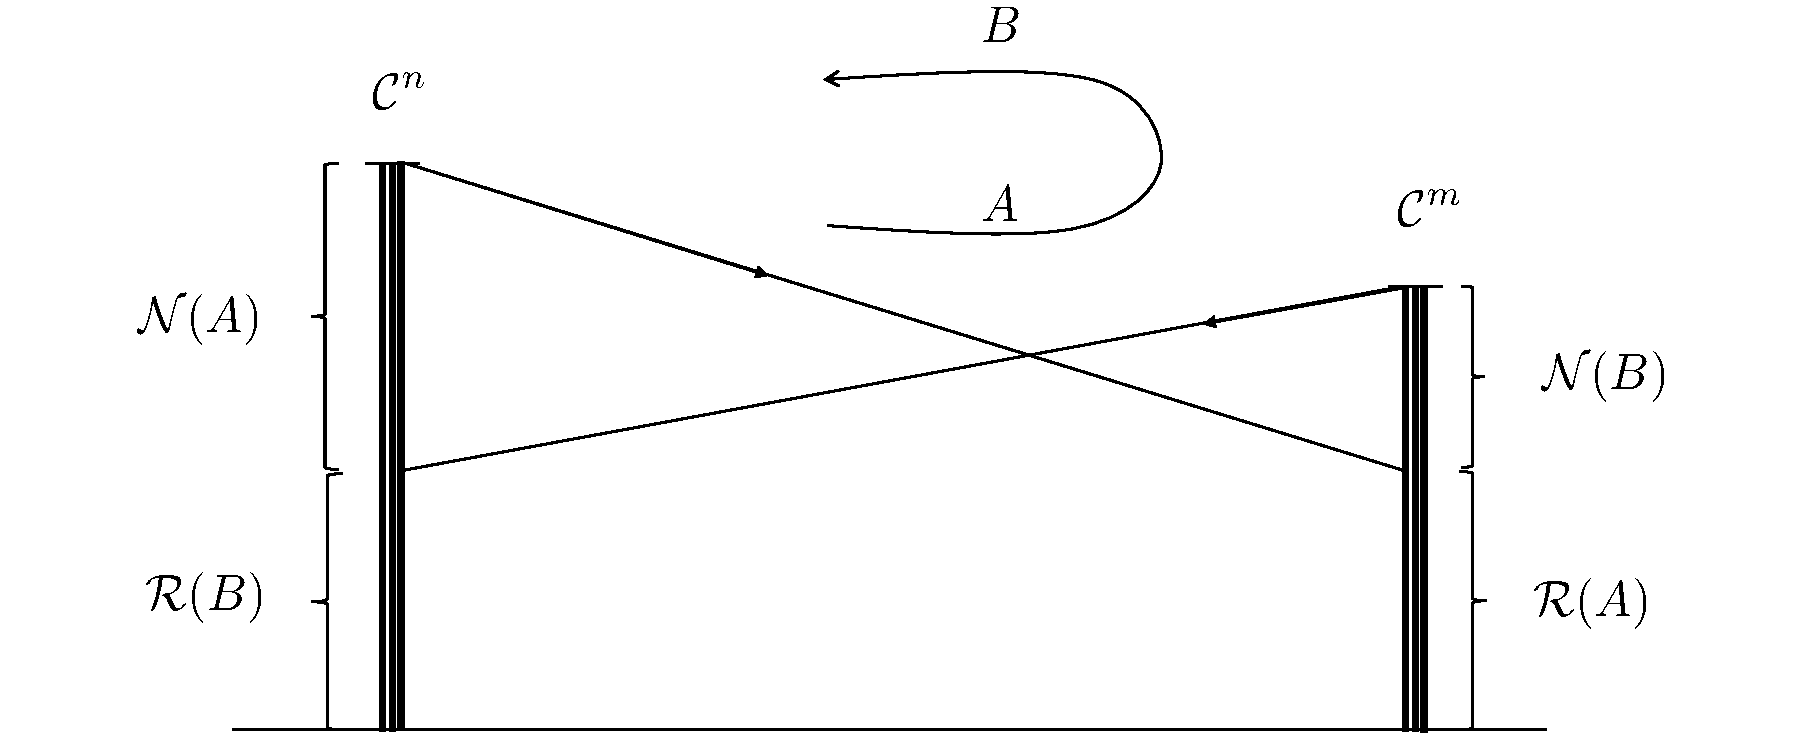
\includegraphics[width=\textwidth]{figures/chap4_left_inverse}	
			\end{center}
			\begin{center}	
	  			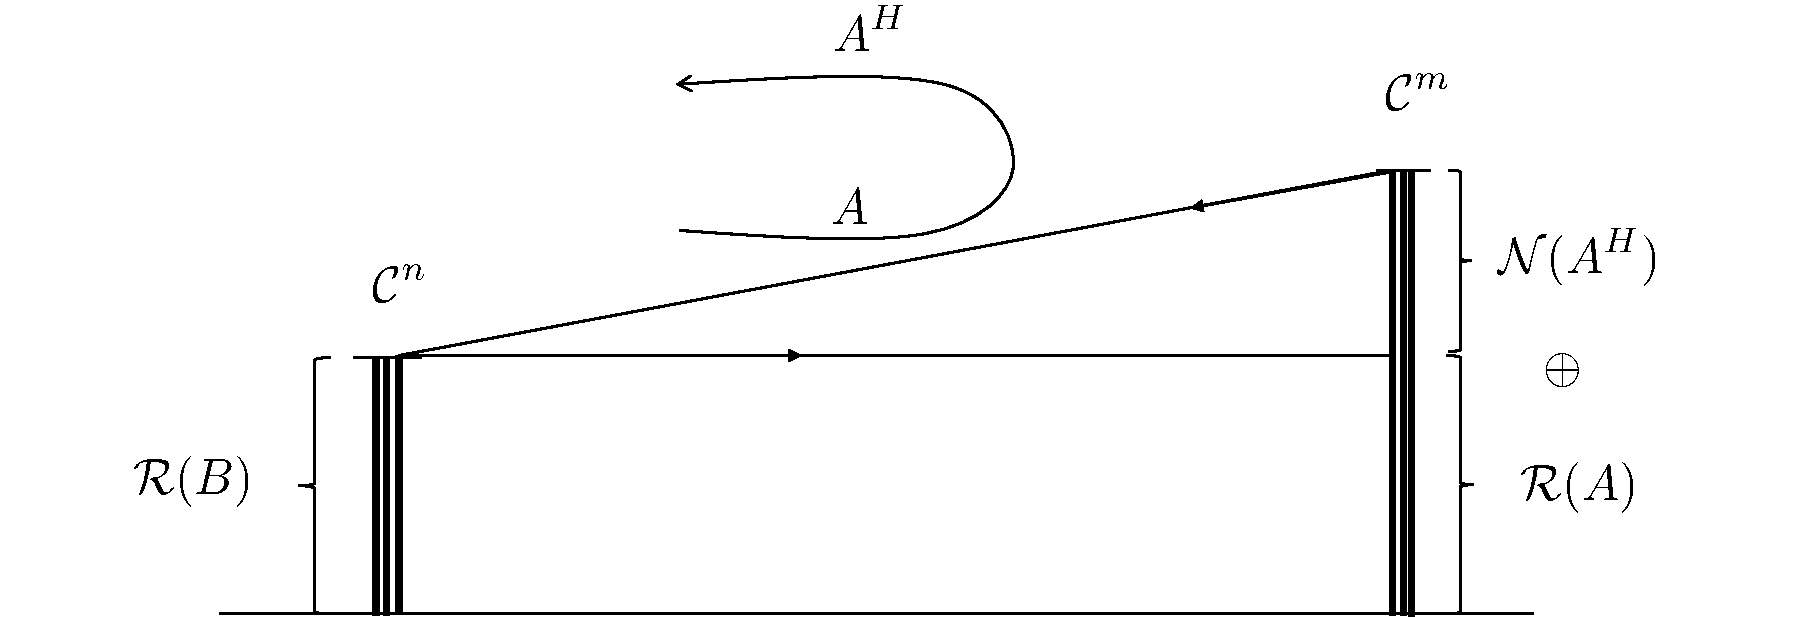
\includegraphics[width=\textwidth]{figures/chap4_left_inverse_full_rank}
			\end{center}
		\end{column}
	\end{columns}
\end{frame}

%----------------------------------
\begin{frame}\frametitle{Right Inverse}
	\begin{columns}
		\begin{column}{0.6\textwidth}
			\begin{itemize}
			\item 	Let $D$ be a right inverse of $A$.  
			\item Then $AD=I:\mathbb{C}^m\to\mathbb{C}^m$.  
			\item Of necessity we must have that $\mathcal{N}(A^H) = \{0\}$, otherwise $D^H A^H = I$ is impossible.
			\item 	$\mathcal{N}(A)$ may be nontrivial therefore if $\hat{x}$ is a solutions so is $\hat{x} + x_n$ where $x_n \in \mathcal{N}(A)$ since $A(\hat{x}+x_n) = A\hat{x} = b$.  Therefore, there is \underline{at least one} solution.
			\end{itemize}
		\end{column}
		\begin{column}{0.5\textwidth}
			\begin{center}
	  			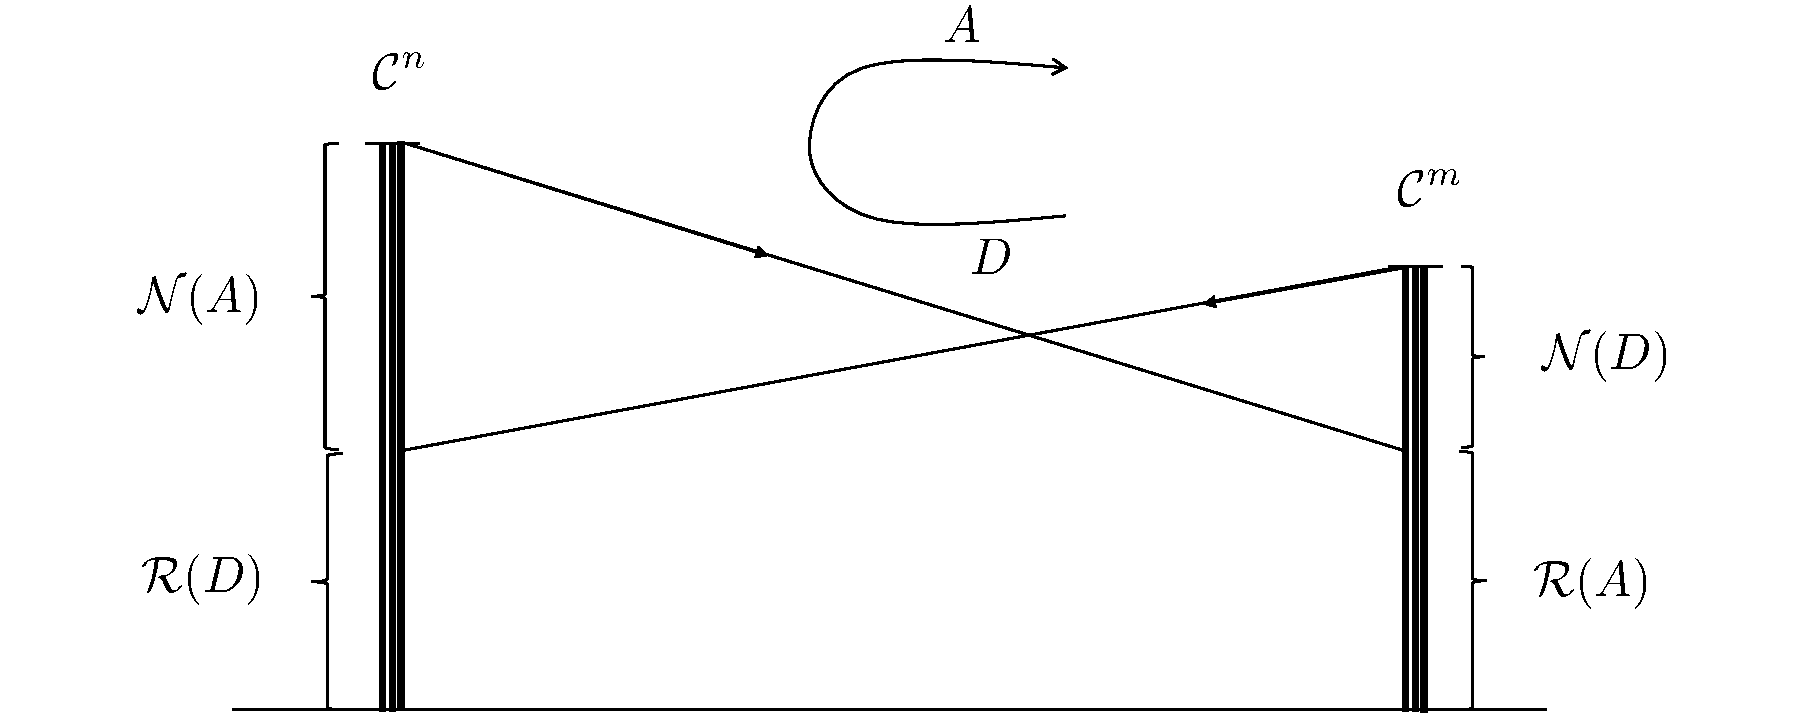
\includegraphics[width=\textwidth]{figures/chap4_right_inverse}	
			\end{center}
			\begin{center}	
	  			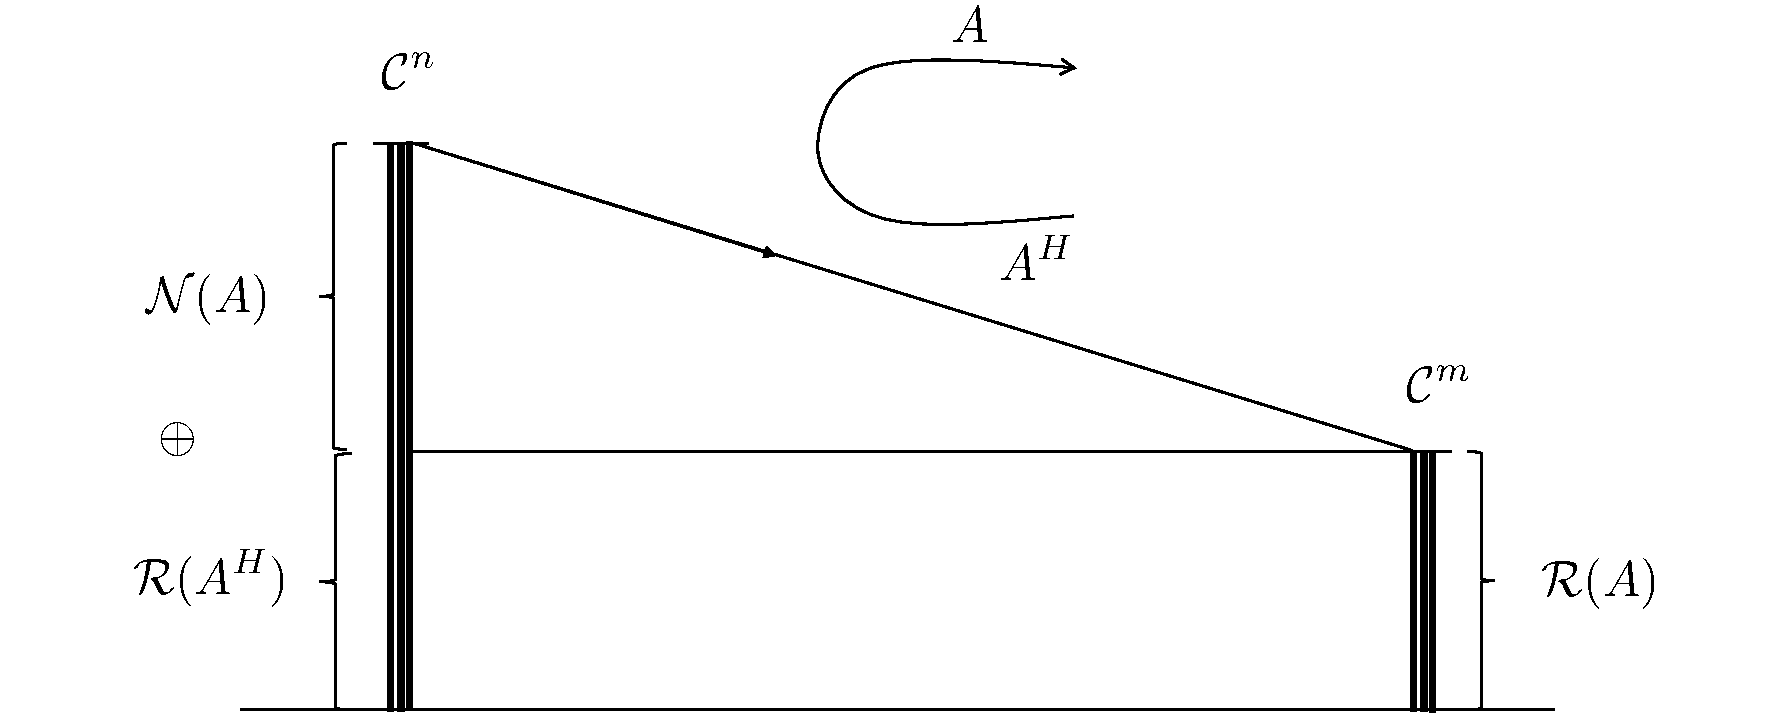
\includegraphics[width=\textwidth]{figures/chap4_right_inverse_full_rank}
			\end{center}
		\end{column}
	\end{columns}
\end{frame}

%----------------------------------
\begin{frame}\frametitle{Right and Left Inverses}
	\begin{lemma}
		\begin{enumerate}
		\item If $A$ has a left inverse then $Ax = b$ has at most one solution.
		\item If $A$ has a right inverse then $Ax = b$ has at least one solution.
		\end{enumerate}
	\end{lemma}
\end{frame}

%----------------------------------
\begin{frame}\frametitle{Regular Inverse}
	If $A \in \mathbb{C}^{n \times n}$ when the following statements are equivalent:
	\begin{enumerate}
  		\item $A^{-1}$ exists
  		\item $\mathcal{N}(A) = \{0\}$ and $\mathcal{N}(A^H)=\{0\}$.
  		\item $rank(A) = n$
  		\item $det(A) \neq 0$
  		\item (right inverse of $A$) = (left inverse of $A$) = $A^{-1}$
  		\item there are no zero eigenvalues of $A$
  		\item $A^HA$ is positive definite
  		\item $A$ is nonsingular
		\end{enumerate}
\end{frame}

%----------------------------------
\begin{frame}\frametitle{Regular Inverse, cont.}
	If $A^{-1}$ exists then 
	\[
	\boxed{A^{-1} = \frac{adj(A)}{det(A)}}
	\]
	where $adj(A)$ is the adjugate of $A$ where $adj(A) = [B_{ij}]^\top$ and $B_{ij} = (-1)^{i+j}det(M_{ij})$ and $M_{ij}$ is the $(i,j)^{th}$ minor of $A$.

	\begin{example}	
		\[ A = 
			\left( 
  			\begin{array}{cc}
    			a & b\\
    			c & d
  			\end{array}
			\right) 
		\]
		\[ adj(A) = 
			\left( 
  			\begin{array}{cc}
    			(-1)^2|d| & (-1)^3|c|\\
    			(-1)^3|b| & (-1)^4|a|
  			\end{array}
			\right)
		= 
			\left(
  			\begin{array}{cc}
    			d & -c\\
    			-b & a
  			\end{array}
			\right)
		\]
		so
			$A^{-1} = \frac{
			\left( \begin{array}{cc}
			d & -c\\
			-b & a
			\end{array}
			\right)
			}
			{det(A)}
			= \frac{
			\left( \begin{array}{cc}
			d & -c\\
			-b & a
			\end{array} \right)
			}
			{ad - cb}$
	\end{example}
\end{frame}

%----------------------------------
\begin{frame}\frametitle{Matrix Rank}
	\begin{lemma}
		Let $A:\mathbb{C}  ^n \to \mathbb{C}^m$ then
		\[ rank(\underset{m\times n}{A}) = rank(\underset{n \times m}{A^H}) = rank(\underset{n\times n}{A^HA}) = rank(\underset{m\times m}{AA^H}) \]
	\end{lemma}
	
	\begin{proof}
		\begin{align*}
		rank(B) &= \text{ \# of linearly independent columns}
				= \dim(\mathcal{R}(B))\\
				&= \text{ \# of linearly independent rows }
				= \dim(\mathcal{R}(B^H)).
		\end{align*}
		Therefore 
		\begin{align*}
		rank(A) &= \dim(\mathcal{R}(A))
				= \dim(\mathcal{R}(A^H)) = rank(A^H)\\
				&= \dim(\mathcal{R}(AA^H)) =rank(AA^H) \text{ Since $\mathcal{R}(A^\ast) = \mathcal{R}(AA^\ast)$} \\
				&= \dim(\mathcal{R}(A^HA)) = rank(A^HA) \text{ Since $\mathcal{R}(A) = \mathcal{R}(A^\ast A)$}
		\end{align*}
	\end{proof}
\end{frame}

%%----------------------------------
%\begin{frame}\frametitle{Left Inverse: Least Squares}
%	\begin{columns}
%		\begin{column}{0.5\textwidth}
%			\begin{itemize}
%			\item 	Consider the solution of $Ax=b$ where $m>n$, i.e., $A$ is tall.
%			\item Assume $A$ is full rank, i.e., $rank(A)=n$.
%			\item Assume $b \in \mathcal{R}(A)$
%			\end{itemize}
%		\end{column}
%		
%		\begin{column}{0.5\textwidth}
%			\begin{center}
%				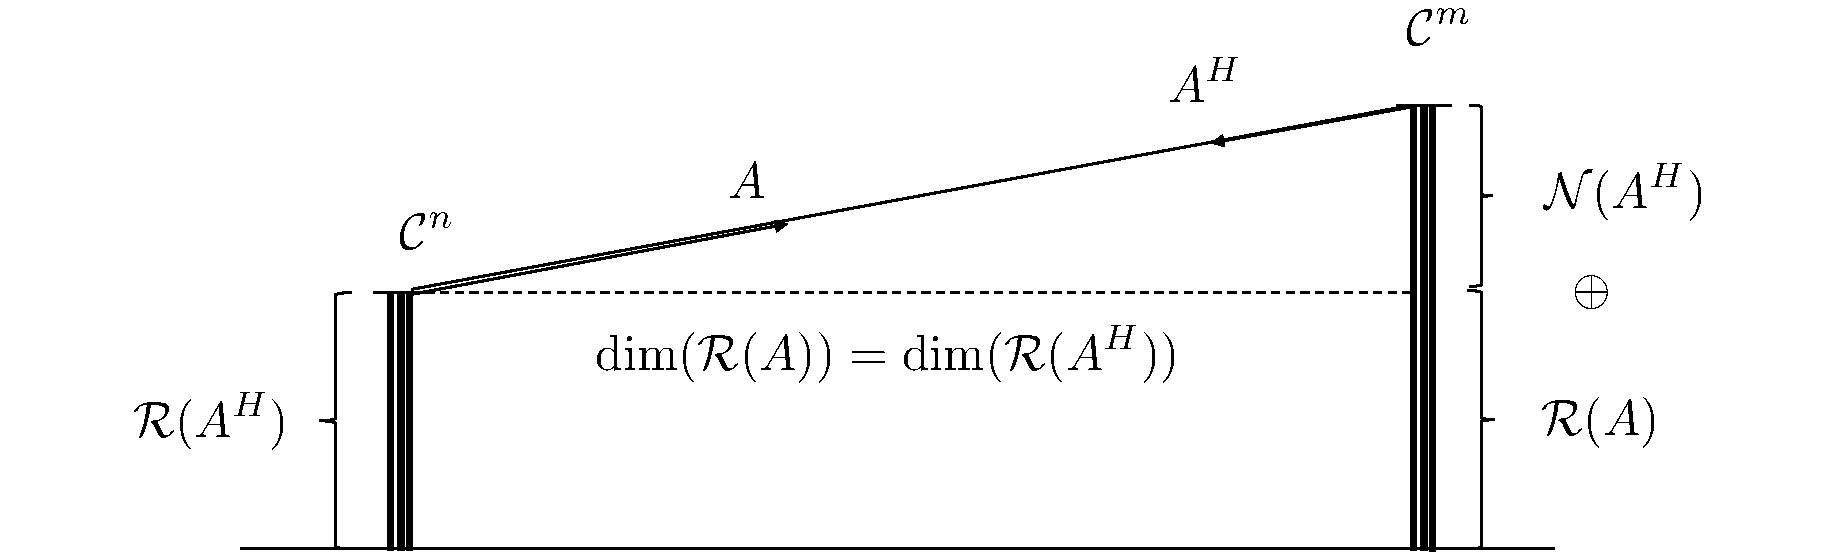
\includegraphics[width=\textwidth]{figures/chap4_least_squares}
%			\end{center}
%		\end{column}
%	\end{columns}
%
%\end{frame}

%----------------------------------
\begin{frame}\frametitle{Left Inverse: Least Squares}
	\begin{itemize}
		\item 	Consider the solution of $Ax=b$ where $m>n$, i.e., $A$ is tall.
		\item Assume $A$ is full rank, i.e., $rank(A)=n$.
		\item Assume $b \in \mathcal{R}(A)$
	\end{itemize}
	\begin{center}
		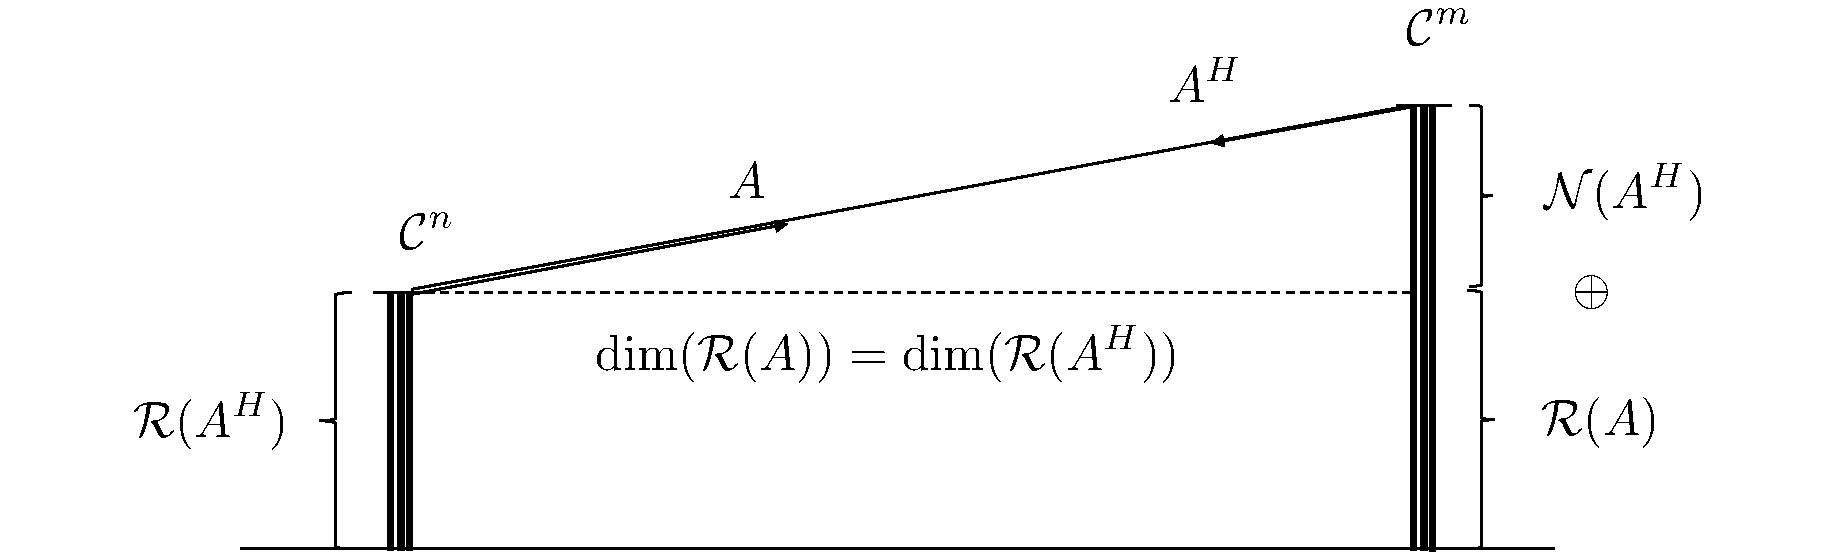
\includegraphics[width=\textwidth]{figures/chap4_least_squares}
	\end{center}
	
	\begin{itemize}
		\item Map $b$ to $\mathcal{R}(A^\ast) :  A^Hb = A^HAx$
		\item Since $rank(A) = n \iff rank(A^HA) = n$ so $(A^HA)^{-1}$ exists
			\[ \Rightarrow \fbox{ $x = (A^HA)^{-1}A^Hb$ } \]
	\end{itemize}
\end{frame}

%----------------------------------
\begin{frame}\frametitle{Left Inverse: Least Squares, cont.}
	What if $b \notin \mathcal{R}(A)$?  This is the least squares problem, e.g.
	\[
	\underbrace{
		\underbrace{
		\begin{pmatrix}
 	   		a_1 & 1\\
  	  		a_2 & 1\\
  	  		\vdots & \vdots \\
   	 		a_n & 1
 	 	\end{pmatrix}
		}_A
		\underbrace{
		\begin{pmatrix}
	  		x_1\\
	  		x_2
		\end{pmatrix}
		}_x
		= \underbrace{
		\begin{pmatrix}
  	  		b_1\\
  	  		\vdots\\
  	  		b_n
  		\end{pmatrix}
  		}_b
		}_{\text{ linear regression }}
	\]

	Since there is no solution, it is reasonable to find $x$ that minimizes $\norm{e}_2$ where
	\[ e = Ax - b \].

\end{frame}

%----------------------------------
\begin{frame}\frametitle{Left Inverse: Least Squares, cont.}
	\begin{itemize}
	\item 	Note that $b = b_r + b_n$ where $b_r \in \mathcal{R}(A)$ and $b_n \in \mathcal{N}(A^H)$ so $e = Ax - b_r - b_n.$
	\item Since $Ax - b_r \in \mathcal{R}(A) \perp \mathcal{N}(A^H)$ the best we can do is make $Ax = b_r \Rightarrow e = b_n$.
	\item Since $b_n \in \mathcal{N}(A^H) $ we have 
		\begin{align*}
			& 0 = A^HAx - A^Hb_r \\
			\Rightarrow & \underbrace{A^HAx}_{\text{projection of $x$ onto $\mathcal{R}(A^H)$}} = A^Hb_r = \underbrace{A^Hb}_{\text{projection of $b$ onto $\mathcal{R}(A^H)$}}
		\end{align*}
	\item Since $rank(A^HA) = rank(A) = n$ we have
		\[\underbrace{x = (A^HA)^{-1}A^Hb}_{\text{least square solution}}\]
	\end{itemize}
\end{frame}

%----------------------------------
\begin{frame}\frametitle{Right Inverse: Min-Norm Solution}
	\begin{itemize}
		\item 	Consider the solution of $Ax=b$ where $m<n$, i.e., $A$ is fat.
		\item Assume $A$ is full rank, i.e., $rank(A)=m$.
	\end{itemize}
	\begin{center}
		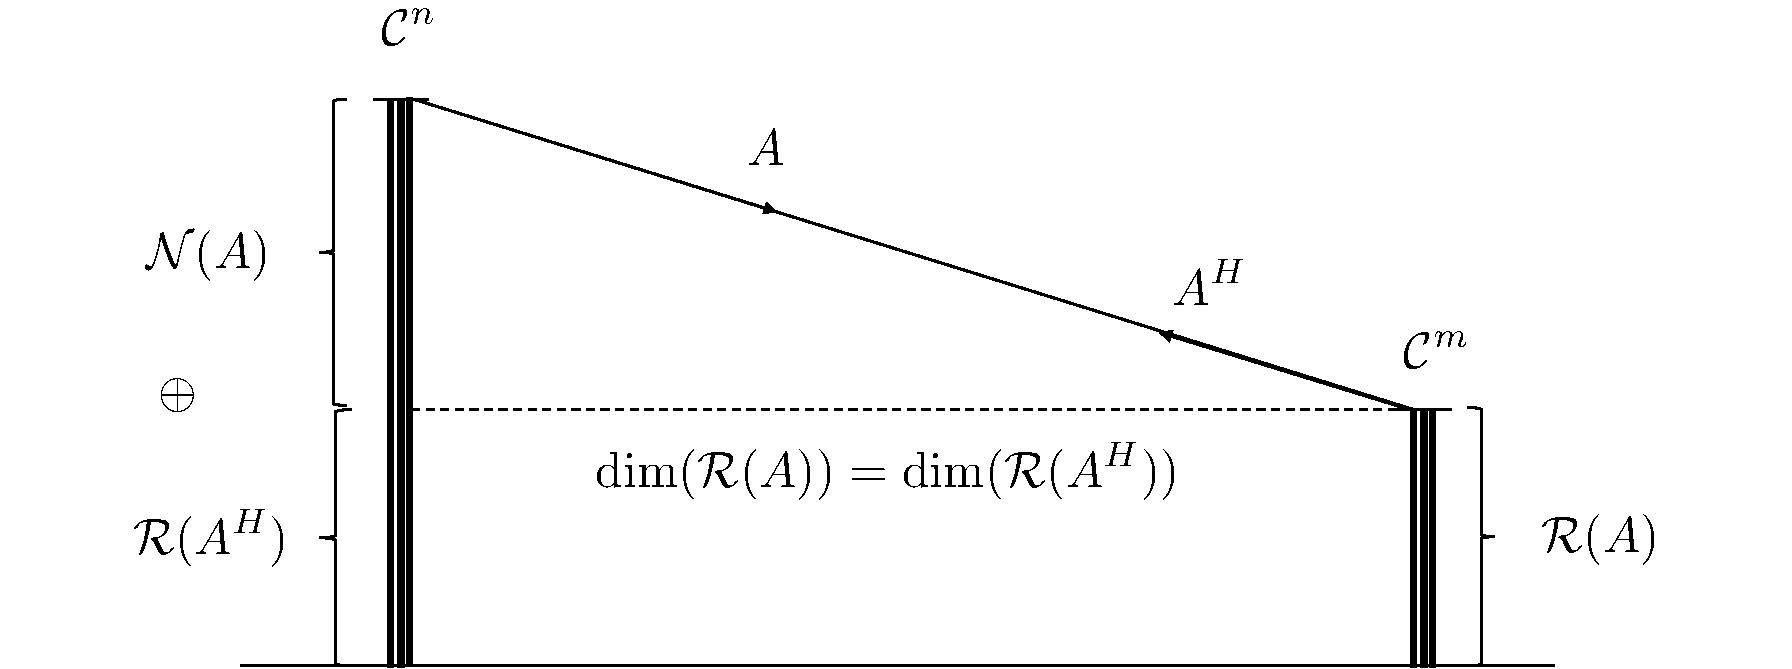
\includegraphics[width=\textwidth]{figures/chap4_min_norm}
	\end{center}
	
	We would like to solve $Ax = b$ note that since $x = x_r + x_n$ where $x_r \in \mathcal{R}(A^H)$ and $x_n \in \mathcal{N}(A)$ and $\mathcal{N}(A) \neq \{0\}$ there are an infinite number of solutions (i.e. add any thing in $\mathcal{N}(A)$ to a solution).  
	The minimum norm solution will be the element of $\mathcal{R}(A^H)$ that satisfies $Ax_r = b$.
\end{frame}

%----------------------------------
\begin{frame}\frametitle{Right Inverse: Min-norm Solution, cont.}
	\[ x_r \in \mathcal{R}(A^H) \Rightarrow x_r = A^Hy \text{ where } y \in \mathbb{C}^m \]
	so we need to solve
	\[ (\underset{m\times n}{A}\underset{n\times m}{A^H})\underset{m\times 1}{y} = \underset{m \times 1}{b} \]
	Since $rank(A) = rank(AA^H) = m$, $(AA^H)^{-1}$ exists.
	\[ \Rightarrow y = (AA^H)^{-1}b \]
	\[ \Rightarrow \fbox{ $x_r = A^H(AA^H)^{-1}b$ } \]
	Note that this is the same solution as
		\begin{mini*}|s|
		{}{\norm{x}_2}{}{}
		\addConstraint{Ax = b}	
		\end{mini*}
\end{frame}

%----------------------------------
\begin{frame}\frametitle{Right and Left Inverses}
	\begin{lemma}
		If $A\in\mathbb{C}^{m\times n}$ where $m>n$ and $A$ is full rank, then 	$ (A^HA)^{-1}A^H $ is a left inverse of $A$.
	\end{lemma}
	\begin{proof}
		$\qquad\qquad\qquad (A^HA)^{-1}A^HA = I_n$
	\end{proof}
	\begin{lemma}
		If $A\in\mathbb{C}^{m\times n}$ where $m<n$ and $A$ is full rank, then 	$A^H(AA^H)^{-1}b $ is a right inverse of $A$.
	\end{lemma}
	\begin{proof}
		$\qquad\qquad\qquad AA^H(AA^H)^{-1} = I_m$
	\end{proof}
	
	\begin{itemize}
		\item Both are examples of pseudo-inverses.
		\item $A^H(AA^H)^{-1}$ is called the Moore-Penrose pseudo-inverse.  
		\item In Matlab type \texttt{pinv(A)}.
	\end{itemize}
\end{frame}




\end{document}